\documentclass[11pt,a4paper]{article}
\usepackage{graphicx} % Required for inserting images
\usepackage{setspace} % For changing line spacing
\usepackage[left=25mm,right=25mm,top=25mm,bottom=25mm,paper=a4paper]{geometry}
\usepackage{amsmath}
\usepackage{hyperref}

\usepackage{graphicx}
\graphicspath{ {figures/} }
\usepackage{array}


\begin{document}
%\linespread{1.25}
\setstretch{1.5}

\thispagestyle{empty}
\null
\vfill
\begin{center}


    {\Large{\bf Missing Data techniques for Reject Inference}} \vspace{0.5cm}


    {\normalsize Master's Thesis submitted\\\vspace{0.5cm}



    {\normalsize by \\\vspace{0.5cm}
    {\bf Radoslav Evtimov} \\
    (570341)} \vspace{1cm}
    }


    {\normalsize in partial fulfillment of the requirements \\
    for the degree of \\
    {\bf Master of Science}


    \vspace{5 cm}
    {\normalsize Chair of Information Systems \\
    School of Business and Economics \\
    Humboldt-Universit\"at zu Berlin 
    } \vspace{1cm}

    First Examiner: Prof. Dr. Stefan Lessmann \\
    Second Examiner: Prof. Dr. Benjamin Fabian

    \vspace{1cm}
    Berlin, March 7, 2024}
    \end{center}

    \newpage




\section*{Abstract}



Reject Inference in credit risk scoring aims at improving the performance of the models used by labeling a subset of the consumer population that would otherwise be isolated from the training process. As the loan repayment datasets only consist of accepts from previous loan application processes, the scoring models end up not being trained on a suitable set of applicants to be representative of the population. Different methods have been proposed for this problem, but more novel approaches from the missing data literature are still to be explored.

The aim of this Master's Thesis is to discover some of the latest developments in the missing data literature and leverage them for a different context - the Reject Inference (RI) problem in the credit risk scoring domain. Through a literature review, the thesis follows the development of the missing data literature and suggests the potential use of newly developed models suiting the Reject Inference sampling bias problem.

It constructs synthetic credit risk data, simulates the credit approval process, and tests techniques for dealing with both MNAR and MAR missingness. Measuring the potential benefits would give a better answer to the question if the missing data literature is applies to the credit risk setting and if yes, aims at answering the question if and which models show a better performance than the conventional RI techniques.

The repository with all scripts used for the thesis as well as results can be found under \url{https://github.com/evtimovr/missing_data_techniques_RI}.

\newpage

% List of figures
\listoffigures


\newpage

\tableofcontents

\newpage

\section{Introduction}

Reject Inference for credit risk scoring proves to be a growingly interesting topic in the credit risk society. Together with the growth in crediting the efforts to improve the credit risk models is a pivotal task possibly resulting in benefits for the financial institutions employing improved models and the economy on its own. 

The issue incepting from not observing the outcome of all applicants remains a challenge for credit risk models. Potential borrowers who are not receiving an approval status in the application process never have the chance to be correctly labeled and thus remain a missing data record. Those are usually completely ignored in the subsequent model optimization, resulting in a significant sampling bias - scoring the overall population of applicants based only on training data from a non-random subset of it. 

The Reject Inference techniques are the answer to the question of what could be a mitigation measure. However, they are hard to test based on real-life data as achieving complete data requires financial institutions to finance applicants with a much higher probability of default (PD), an extremely costly path that would usually not be pursued as a strategy. This drives the community towards other solutions that require modeling for the missing values and aiming at improving the accuracy of the credit risk models without employing any costly operations. Employing missing data techniques is one of the usual approaches, but with the advances in the missing data literature, several of the newer techniques are to be explored and validated in different domains, one of which is credit risk modeling. 

The scope of this thesis is the overview and analysis of several of the existing methods. To achieve this, this thesis uses simulated data.


\section{Background}


\subsection{Missing data mechanisms}

Rubin and Little's work (\cite{rubin1987multiple,rubin1976inference}) introduced a framework for missing data mechanisms in an effort to understand how to approach the missing data problem. They have defined three types of missingness depending on the relationship between the missing and observed data. The \textit{Missing Completely at Random (MCAR)} defines a situation where the missing data is completely independent of the observed variables. As per  \cite{ehrhardt_reject_2021} that looks at the missingness mechanism from the Reject Inference perspective. 

In a case where Z is the financing mechanism, Y the repayment status, and X contains the features of an application, in the MCAR case, Z is independent from X and Y: 

$$
\forall \boldsymbol{x}, y, z, p(z \mid \boldsymbol{x}, y)=p(z)
$$

Usually, this type of missingness is perceived as harmless and often ignorable. 
The \textit{Missing at Random (MAR)} mechanism defines a case where the missingness depends only on the observed data points and not on the repayment \textit{Y}, whereas the \textit{Missing Not at Random (MNAR)} mechanism is the case where $Z$ depends on $X$ and $Y$. 
$$
\begin{aligned}
MAR \quad
\forall \boldsymbol{x}, y, z, p(z \mid \boldsymbol{x}, y)=p(z\mid \boldsymbol{x})
\end{aligned}
$$
$$
\begin{aligned}
MNAR \quad
\exists \boldsymbol{x}, y, z, p(z \mid \boldsymbol{x}, y)!=p(z\mid \boldsymbol{x})
\end{aligned}
$$

$MAR$ and $MNAR$ are the subject of serious attention and many methods deal with them as they require treatment and can’t be ignored if one wants to avoid biased results. 

\subsection{Credit risk scoring}

The financial institutions and the risks they take play a crucial role in the modern day's economy. They are often in the focus exactly because of the imbalanced risk they take when allocating capital. In the setting of retail banking, a loan is usually allocated in several steps: 

\begin{enumerate}
  \item A customer requests a loan and submits documentation
  \item The customer's documentation and externally collected data form a dataset that is used for evaluation
  \item A scoring model evaluates the \textit{Probability of Default (PD)} of the customer
  \item Based on the results of the model and a given threshold (symbolising the risk appetite) a loan is allocated or not
\end{enumerate}

The people receiving a loan would be called \textit{accepts} and the ones declined - \textit{rejects}.

Because of the crucial role those models play, they are under close supervision from regulators and state authorities. This process prevents banks from unnecessary risks and ensures profitability. From a societal point of view, the credit risk models ensure the non-risky allocation of resources, and from the bank's view they lower the probability of loss. 
As financial institutions' (except special institutions like state-owned banks) primary goal is profit and would usually prefer losing a customer rather than a failing loan. 

\subsection{Reject Inference}

Emphasizing the importance of the credit risk models, it is clear it is of utmost importance to maintain the models used to a high level of accuracy as often decisions are taken solely on their results. It is important to note that sometimes there are factors not measurable in a quantitative way that influence the decision of the bank. In a physical bank, this might be a subjective impression or opinion by a credit consultant. This might lead to a difference in the features influencing the financing decision and the repayment.

Lenders train the models used only on the outcome data of already approved applicants. This leads to a sample bias and a deterioration of the model performance as the new applicants are scored on models trained on a non-representative population. This sampling bias leads to performance deterioration over time with some customers remaining underfinanced and the banks potentially declining good customers which could provide additional profit. All techniques dealing with this problem are encompassed by the term \textit{Reject Inference (RI)}. 
\textit{RI} aims to improve the performance of credit scoring models by obtaining the missing repayment labels for the rejected applicants. The assumption is the more available data, the better the performance of the model trained on it. 

Some of the pain points and the criticism on Reject Inference as a set of techniques are well summarised by \cite{kozodoi2020shallow}. Empirical evidence about the value of RI and its efficiency is scarce. Most studies only work with accepted cases (\cite{Banasik_Crook_2010}), do not possess an unbiased sample with accepts and rejects (\cite{Bücker_Van_Kampen_Krämer_2013}) or use synthetic data. This is mainly due to the unavailability of data of this kind. Apart from that, most studies focus on linear models of SVMs (support vector machines), while there are already techniques showing better performance in the field (\cite{Lessmann_Baesens_Seow_Thomas_2015}). 

It is important to mention the two different issues Reject Inference is trying to deal with. One of them is model performance - the models using data with sampling bias are meant to perform worse than they could be with complete data. But also model evaluation - the issue of choosing the best model. The performance of models has usually been evaluated on an "incomplete" dataset which leads to wrong conclusions when making decisions in this regard. 

Another important consideration in RI, but also in credit risk scoring in general is the regulatory environment around the used models. They should per regulation be strictly monitored, but also easy to justify and explain whenever requested. The scrutiny of regulators and society pushes financial institutions into a dilemma of what models exactly to use, but often also takes away some of the potential options the research has been looking at. RI techniques, whatever they are, should be able to also withhold this challenge to be practically successful.

\subsubsection{MAR vs. MNAR}
The question of whether Reject Inference deals with a MAR or an MNAR problem is one with no clear answer. In the general missing data literature, it is fairly hard to estimate what kind of missing mechanism there exactly is and this is often the judgement of experts. In the case of Reject Inference as per \cite{gongyuebound} the missingness mechanism in the credit scoring depends on what one believes about the classification performance of the used credit scoring models - if the assumption is they perform well, Reject Inference could be classified as a missing data problem between MAR and MNAR as it depends on both \textit{Xs} and the missing data itself - the \textit{Y} outcome. 


\section{Literature review}

The following section will encompass the most important developments in the field of missing data research and will only later focus on its application in the reject inference setting. 


Missing data techniques develop constantly as the topic is of utmost importance to better understand and tackle, but a recent review of published machine learning applications suggests that the majority of studies use deletion methods for their missing data handling, despite many software packages offering better alternatives \cite{Nijman_Leeuwenberg_Beekers_Verkouter_Jacobs_Bots_Asselbergs_Moons_Debray_2022}. 

In his book \cite{enders2022applied} Enders looks at missing data from the perspective of what he calls three analytical pillars of missing data. Those are maximum likelihood, Bayesian estimation, and multiple imputation. This literature review will therefore follow the structure of those three pillars.  

\subsection{Maximum Likelihood estimation (MLE)}

While the origins of maximum likelihood missing data handling date to the 1950s, the first became practically usable in the 1990s when software advancements started allowing its implementation. The classical MLE aims at optimizing parameters so that a minimum squared standardised difference between real-world data and the predictions is achieved. In the missing data use case, a log-likelihood equation is maximized assuming all the observations share the same model parameters while the contribution of each is limited only to the observed data points\cite{enders_missing_2023}. Even though the result is not an actual imputation, the location of the missing data point is inferred from the probability estimator. 

An important topic around the MLE remains its robustness to nonnormal data. Simulation work on the matter has proven MLE to be consistent in many applications, but missing data could distort approximate fit indices even with normal data \cite{Zhang_Savalei_2023}. A topic that has developed in the last decade is the maximum likelihood estimators for factored regression specifications\cite{enders_missing_2023}. Flexible approaches that accommodate mixtures of categorical and continuous variables in terms of factorisation are available, but there are still not all combinations of metrics available \cite{Rabe-Hesketh_Skrondal_Pickles_2004, ludtke2020analysis}. 

\subsection{Bayesian Estimation}

The Bayesian paradigm considers parameters as random variables and the posterior encompasses our subjective knowledge about the potential realisation while collecting more data. The development in the Bayesian estimation techniques used for handling missing data has outpaced the maximum likelihood methods in the last two decades \cite{enders_missing_2023}. Initially, the multivariate normal distribution was the predominantly used Bayesian model and the natural fit of Bayesian estimation with factored regression specification makes it a popular solution for this setting. 

Interesting advancements in the factored regression specifications setting include latent variable models. \cite{ludtke2020regression,kellerblimp,merkle2015blavaan}, models for missing not at random processes \cite{du2022bayesian}, auxiliary variable models \cite{daniels2014fully}, multilevel models \cite{grund2016multiple, enders2020model}). 

\subsection{Multiple Imputation}

Multiple imputation \cite{rubin1976inference} is a method that includes an imputation phase, an analysis phase, and a pooling phase. First, the values are imputed iteratively, then the imputations are used for analysis as if the preferred method can leverage a complete dataset and finally, the imputations from all iterations are combined to present a single set of results using standard combining rules introduced by Rubin.

Descriptions of the classic procedure are described in multiple research papers including \cite{schafer_missing_2002}. There is plenty of literature focusing on ways to deal with the imputation of nonnormal data by transformation prior imputation - methods like Box–Cox, logarithmic, square root, inverse, fourth-root, and logit transformations, among others \cite{enders_missing_2023, van2018flexible, von2009impute, lee2017multiple}. \cite{enders_missing_2023}

Another set of research papers works on generating nonnormal imputations. As an example, the predictive mean matching uses the classic method, but draws from a pool of observations whose prediction is similar to the missing data sample \cite{van2018flexible, kleinke2017multiple}. 

When talking about categorical missing variables, initially the research community was using the normal imputation models by rounding the continuous imputation value to a discrete value. Nowadays there are much more suitable ways of dealing with this - the use of a latent response framework to adapt binary, ordinal, and multicategorical nominal variables \cite{asparouhov2010multiple, quartagno2019multiple}. 

An important development in the field of multiple imputation is the introduction of the fully conditional specification. The idea here is to use a sequence of univariate regression models to impute variables one at a time instead of using a multivariate distribution \cite{van_buuren_multiple_2007,van2018flexible}). In this case, each regression is tailored to the incomplete variables metric allowing for a diverse collection of generalized linear models \cite{enders_missing_2023}. There have been further developments using the framework of Van Buuren and extending it to incomplete covariates, multilevel data structures, classification and regression trees, and regularised regression.

Potential issues with the fully conditional specification are flagged by \cite{bartlett2015multiple, liu2017evaluation} and mainly focus on the fact that univariate conditional distribution in certain cases cannot derive from the same multivariate distribution. An example of this is when the model features incomplete interactive or nonlinear effects. In a case like this, even if the missing at random condition is satisfied, approaches based on just-another-variable imputation can produce substantial bias (Kim et al., 2015, 2018).\cite{kim2015evaluating}



\subsection{Missing Not At Random}

The literature around handling Missing Not at Random (MNAR) data encompasses mainly two approaches - selection models and pattern mixture models. They both introduce a model that describes the occurrence of missing data in their effort to fight nonresponse bias. The approach of using an indication of missing data is typical for both approaches, but they are used in completely different ways - the selection model uses the indicator as a dependent variable in a regression while the pattern mixture models leverage it as a predictor. 

\cite{enders_missing_2023} points out selection models and pattern mixture models are underutilized as software tools are no longer a barrier to implementation and researchers have multiple options as it has never been easier to fit those models from a computational point of view. The pattern mixture models are usually used for the analysis of data measured over time to population-level change and individual differences in change characteristics \cite{xu_sensitivity_2011}.  

Wu \& Carroll \cite{wu1988estimation} provide a discussion on using one or more latent variables predicting missingness.
In recent years there have been graphical methods developed to study parameter recovery. Examples are \cite{mohan2021graphical, mohan2013graphical}, their work aims at supporting the evaluation if MNAR data analysis can produce meaningful estimates. 

A recent contribution to the MNAR data imputation is the work of \cite{peng_handling_2023} that develops a Monte Carlo likelihood approach in correcting the bias in parameter estimation using expectation maximization (EM) to overcome computational issues other approaches previously had.


More will be elaborated on two models - \cite{galimard_heckman_2018} and \cite{Andridge_Little_2020} in the following sections. They are good representatives of both primary approaches in dealing with MNAR missingness - selection models and pattern mixture models. 


\subsection{Multilevel data}

Multilevel data is also known as hierarchical or nested data and describes data structure where observations are nested within higher-level units, which leads to dependencies or correlations within the same group. \cite{xu_sensitivity_2011} 

All three analytical pillars in the missing data literature have been extended in recent decades to accommodate the multilevel data setting. Papers that give a good summary of those developments are \cite{enders2022applied,grund2016multiple,grund2021treatment}.

The multilevel setting is usually tackled by random intercept models and the literature suggests that maximum likelihood is the most suitable approach for this \cite{enders_missing_2023}. The popular joint model imputation of Joseph Schafer \cite{olsen_two-part_2001} was extended to multilevel data structures. Newer approaches like \cite{asparouhov2010multiple} use incomplete categorical variables as well as missing data at any level of the data hierarchy.  Most implementations of the framework only work with a random intercept and cannot account for relationships between the incomplete variables. 

Similar to that, there were also recent developments in Van Buuren’s fully conditional specification. They are also reserved for random intercept models as it fails to capture heteroscedastic variation in the conditional distribution of random slope predictors \cite{enders2020model}. Fully conditional specification and joint model imputation have both shown to be equally effective when applied to random intercept models. A good example of the MNAR missingness model is \cite{hammon_multiple_2020}. The paper leverages what is already developed by \cite{galimard_heckman_2018} and targets a multilevel data setting.


\section{Missing data techniques for Reject Inference}

The following section aims at presenting models suitable for the Reject Inference setting that are implemented as part of \ref{simstudy}. Those are models that represent the main ideas of more advanced techniques for dealing with MNAR data. \textit{MiceMNAR} representing the ideas of a Hacman's selection models and \textit{PPMM} from the family of the pattern mixture models. 

\subsection{Heckman imputation models for binary outcomes}

\subsubsection{Multiple imputation using Heckman's one-step ML estimation  (MIHEml)}


This missing data technique that is coming from the work of Galimard\cite{galimard_heckman_2018}. 

In a research paper from 2018\cite{galimard_heckman_2018}, Galimard et. al develop an algorithm and corresponding R package aiming at leveraging the MICE (multiple imputation by chained equations) method developed by Van Buuren\cite{van_buuren_multiple_2007} to impute binary MNAR missing outcomes. This setting exactly replicates the reject inference use case because of the binary character of the credit risk outcome variables (0 - low probability of default, 1 - high probability of default). 

Their work aims at introducing a method using a sample selection model to impute missing binary outcomes based on a bivariate probit model associated with a one-step maximum likelihood estimator for the first time. Once defined, this model is leveraged in a MICE procedure.

As mentioned in the previous section, there are two main methods for dealing with MNAR missingness. Galimard et. al \cite{galimard_heckman_2018} focus on the first one - selection models. The idea behind Heckman’s selection model is that assuming an MNAR missingness, the conditional expectations of the observed and missing Y are different. 


$$
\begin{aligned}
& R_{y i}^{\prime}=X_i^s \beta^s+\varepsilon_i^s \\
& Y_i^{\prime}=X_i \beta+\varepsilon_i
\end{aligned}  \text {, with }\left(\begin{array}{l}
\varepsilon^s \\
\varepsilon
\end{array}\right) \sim N\left(\left(\begin{array}{l}
0 \\
0
\end{array}\right),\left(\begin{array}{ll}
1 & \rho \\
\rho & 1
\end{array}\right)\right)
$$


Where $R_{y i}$ is an indicator of the missingness of $Y_i$. The model uses the idea of a bivariate probit model, modeling the MNAR missingness based on the error terms between the two equations: the selection equation and the output equation. Those error terms follow a bivariate normal distribution. 

The missingness mechanism is controlled by the correlation coefficient $\rho$. In the case where $\rho$ = 0 the two equations have independent error terms and indicate a MAR (Missing At Random) missingness. In the opposite case, the missingness R depends on Y and thus implies an MNAR (Missing Not At Random) mechanism.

An important note about the model is Heckman’s model must avoid collinearity between the predictors of the two equations, meaning ideally the variables in the two equations would not be exactly the same and the selection equation would have at least one more covariate. An equivalent of this in the Reject inference would imply the selection and the outcome depend on different features of the applicants and a situation like this would be one where there are factors outside of the usual dataset that influence the decision of credit approval. 

Under the MAR mechanism, imputation approaches use the conditional distribution of observed Y given the other covariates to impute the missing Y. In the case of MNAR, however, one would need to model this in another way with the conditional expectations of the observed and missing Y being different. For the binary outcome \cite{Webel_2011}:

$$
P\left(Y_i=1 \mid X_i, X_i^s, R_{y i}=0\right)=\frac{\Phi_2\left(X_i \beta,-X_i^s \beta^s,-\rho\right)}{\Phi\left(-X_i^s \beta^s\right)}
$$


The model for binary outcome missing variables is described in those 3 steps:

The estimated parameter is denoted as $\hat{\theta}$.

The parameter is estimated to be $\theta \sim \hat{\theta}$.

\begin{enumerate}
  \item Use the one-step estimator to obtain Heckman's model parameters ($\hat{\theta},\hat{\Psi}$) where $\hat{\Psi}$ is the variance-covariance matrix of $\hat{\theta}$
  \item Draw $\theta^{*}$ from N($\hat{\theta},\hat{\Psi}$)
  \item Draw $Y_i^*$ from a Bernoulli distribution with parameter $p_i^*$ from:  
\end{enumerate}

$$\rho_i^* = \frac{\Phi_2\left(X_i \beta^*,-X_i^s \beta^{s*},-\rho^*\right)}{\Phi\left(-X_i^s \beta^{s*}\right)}$$



\subsubsection{Multiple Imputation by chained equations (MICE)}

The final step consists of imputing MNAR outcomes and MAR predictors using the MICE framework \cite{van_buuren_multiple_2007}. The idea of the framework is to start by imputing a random observed value, followed by obtaining the posterior predictive distribution of the first missing variable, and then on an iterated sequence filling in the following missing variables by the already imputed values. In the case of one missing variable, the "chained equations" part of the method is skipped. 

The final output of the model is usually an M number of complete datasets (M represents the number of iterations). The analysis is then usually performed after the "pooling phase" of MICE, where the results from any analysis on the imputed datasets are combined using Rubin's rules.
More details on the exact implementation can be found in the following section.


\subsection{Proxy Pattern-Mixture Model}


Another method that will be closely looked at in the current study is the "Proxy Pattern-Mixture Analysis for a Binary Variable Subject to Nonresponse" \cite{Andridge_Little_2020}. This paper looks at extending the already existing work in the proxy pattern-mixture modeling (PMM) to binary variables \cite{Andridge_2011}. 

The main idea in the research paper is to create an algorithm that could enable the evaluation of the potential impact of nonresponse on survey estimates assuming they could also be MNAR rather than the usual assumption missing survey responses are usually MAR. The developed method enables three different versions for evaluation - Maximum likelihood, Bayesian, and Multiple imputation. 

For the Reject Inference use case, we would leverage the multiple imputation (MI) estimation, basing the MI on the specified proxy pattern mixture model (PPMM) to impute the missing values and measure the model improvement using this method. More details on the exact approach will be given in the following section.  


As mentioned before, there are two main approaches for modeling MNAR missing data. The selection models, implemented by \cite{galimard_heckman_2018} and already explained in the previous section. The second approach is the pattern-mixture model (PPM). 

While selection models factor the joint distribution of $M_i$ and $Y_i$ as 

$$
f\left(M_i, Y_i \mid Z_i, \theta, \psi\right)=f\left(Y_i \mid Z_i, \theta\right) f\left(M_i, \mid Z_i, Y_i, \psi\right)
$$

the case in the pattern mixture models looks differently: 

$$
f\left(M_i, Y_i \mid Z_i, \xi, \omega\right)=f\left(Y_i \mid Z_i, M_i, \xi\right) f\left(M_i, \mid Z_i, \omega\right)
$$

where the first distribution on the right-hand side models the distribution of $Y_i$ given covariates $Z_i$ in the different pattern of missingness $M_i$ and the second models the probabilities of different pattern $M_i$.

An important difference between the two is that the Selection model, first defined in \cite{heckman1976common}, requires specifying the missingness model via the density, while the pattern-mixture model, which is the basis for the proposed approach, doesn't require any explicit parametric model for the missingness mechanism. The main interest of the work of \cite{Andridge_2011} is to assess the impact on inference for the proportion of units with Y=1 (target variable). 

The framework assumes that Y (target variable with missing values) is related to a normally distributed latent variable U, so that Y=1 when $U> 0$. Similar to previous approaches from the PPM frameworks by % cite two papers by Andridge
the covariates Z are reduced to a proxy X. Denoting the missingness indicator by M (M=1 when Y is missing), the regression of Y on Z is: 
$$ Pr\left( Y=1\mid Z, M=0\right) = \Phi \left(\alpha_0 + \alpha Z \right) $$

Then after a definition of the pattern-mixture model where we assume the joint distribution of [U,X,M] follows the model discussed in %cite Little (1994)

Of primary interest in the overall model is the marginal mean of Y which can be obtained by averaging over the two patterns (m = 0,1). The estimation looks like this: 

% to be fixed
$$
\begin{aligned}
\mu_y=\operatorname{Pr}(Y=1) & =\operatorname{Pr}(U>0) \\
& =\operatorname{Pr}(U>0 \mid M=0) \times \operatorname{Pr}(M=0)+\operatorname{Pr}(U>0 \mid M=1) \times \operatorname{Pr}(M=1) \\
& =\pi \Phi\left(\mu_u^{(0)} / \sqrt{\sigma_{u u}^{(0)}}\right)+(1-\pi) \Phi\left(\mu_u^{(1)} / \sqrt{\sigma_{u u}^{(1)}}\right)
\end{aligned}
$$

As one can't estimate the parameters $\mu_u, \sigma_uu, \rho$ for the nonrespondents, the model remains underidentified. A $\rho$ indicates the correlation between the latent variable U and X. This correlation is defined for the respondents (M=0) and is called "strength of the proxy", indicating a stronger prediction power of the covariates Z of Y in the probit model. 

In order to obtain $\mu_u^{(1)}, \sigma_{u u}^{(1)}, \rho^{(1)}$ the parameter restrictions from %(Little 1994; Andridge and Little 2011) 
are used, especially the assumption that the M=1 probability is an unspecified function f of the linear combination of X and U: 

$$\operatorname{Pr}(Y=1\mid U,X) = f\left(\left(1-\phi \right) X^{*} + \phi U \right)$$

where $\phi$ is a sensitivity parameter ranging from 0 to 1 that determines the missingness mechanism, the higher the $\phi$, the lower the dependency of Y on the proxy X. For example, a $\phi$ = 0 indicates a MAR missingness, while a $\phi$ = 1 indicates strong MNAR mechanism. A $\phi$ of 0.5 would indicate an equal weight of X and U in their contribution to Y. 

An MNAR case would result in missingness that is a function of U, allowing for "smooth" missingness, which may lie on a continuum instead of only taking two values, as would be the case if missingness depended on Y itself.

The final estimates based on the pattern-mixture model are obtained from three techniques popular in the missing data literature - maximum likelihood, Bayesian inference, and multiple imputation. The choice of technique for the simulation study will be discussed in detail in the next section. 

\section{Simulation study} \label{simstudy}

\subsection{Synthetic Data Generation} \label{data_gen}

Reject Inference (RI) as a process concerns credit risk data and naturally, there are very few completely labeled datasets available as few financial institutions would risk their capital to acquire correct labels. This is one of the reasons why research on the topic is primarily done on synthetically generated datasets. In the case of this simulation study, this will also be the case. 

Usually, RI simulated data draws the values for \textit{good} applicants (the ones who will repay the loan) and \textit{bad} applicants (the ones who will not repay the loan) from two different Gaussian distributions. In this case, we will make use of a similar approach that was already used in \cite{maldonado2010semi}, \cite{ehrhardt_reject_2021}
and \cite{hoffmann2007inferring}. % Cite Lessmann here as well


$$
\begin{cases}x^g \sim \mathcal{N}\left(\mu^g, \Sigma^g\right) & , \text { where } \mu^g \in \mathbb{R}^k \text { and } \Sigma^g \in \mathbb{R}^{k \times k} \\ x^b \sim \mathcal{N}\left(\mu^b, \Sigma^b\right) & , \text { where } \mu^b \in \mathbb{R}^k \text { and } \Sigma^b \in \mathbb{R}^{k \times k}
\end{cases}
$$

where $x^b$ and $x^g$ represent the covariates of the bad and good applicants respectively. Assuming their attributes differ in such a way would provide for a simple and reliable analysis. Additionally to that, a holdout set drawn from the same Gaussian distributions is drawn in order to obtain a dataset for performance evaluation. 

To perform also a sensitivity analysis, variations of this approach will be tried out. To make the task more complex there is the option to draw the \textit{good} and \textit{bad} samples from a mixture of Gaussian distributions, where the final value for variable $X_1$, for example, will be the weighted sum of two different Gaussian distributions. 

$$ 
\begin{cases}
x^g \sim \sum_{i=c}^{C} \pi_c \cdot \mathcal{N}\left(\mu^g, \Sigma^g\right) \\
x^b \sim \sum_{i=c}^{C} \pi_c \cdot \mathcal{N}\left(\mu^b, \Sigma^b\right)
\end{cases}
$$

where $\pi$ represents the weight of each of the Gaussian distribution drawn from. Similar to \cite{Lessmann} two noisy features are added to make the task more complicated. Both belong to the same distribution 
$x_n \sim \mathcal{N}\left(0, 1\right)$. 


\subsection{Proxy Pattern-Mixture Model} \label{ppma}

As explained in the previous section, Aldrigde et. al \cite{Andridge_Little_2020}
use three different techniques to get bias estimates from their pattern mixture model. The primary purpose of their work was to give a good estimate of how harmful the missing data is for their survey data. The primary focus of this work is slightly different - to test any techniques that might improve the performance of credit risk models by reducing the sampling bias in the dataset used. Hence, the technique that was leveraged by the simulation study here is the multiple imputation. 

Even though only a possible step in the original work of \cite{Andridge_Little_2020}
multiple imputation could be used to extract actual imputed values based on the pattern mixture model. In more detail, this simulation study uses the R function documented in the original paper which can also be found at https://github.com/randridge/PPMA. 

Leveraging the already existing MI (multiple imputation) function based on the pattern mixture model as defined in \cite{Andridge_Little_2020} one could get each imputation value for each of the variables. Because of the difference of the use case, a reformatting is needed to reach a format similar to the one used in the mice package in R. The result that is aimed for is an object with all the imputed values per imputation cycle. Such an object is of class "mids" - a class specific to the mice package. The "mids" object allows one to run an analysis of the actual results of an imputation. The analysis this simulation study is aiming for consists of: 


\begin{itemize}
  \item Convert the output of the "mi" function into a mids object
  \item Build logistic regressions over each of the imputed datasets
  \item Use the created models to predict on a test dataset
  \item Pool the results from each imputation into a single set of results
  \item Evaluate the created model on the evaluation measure of choice
\end{itemize}


\subsection{Heckman imputation models for binary outcomes (miceMNAR)} \label{micemnar}

The implementation of the model of Galimard et. al \cite{galimard_heckman_2018} has been done with the help of the miceMNAR package in R. The package is currently not live on CRAN, but could be downloaded from the CRAN archive and installed locally. 

The package contains multiple functions for both binary and continuous variables. The function of interest, \textit{mice.impute.heckprob}, provides an imputation model for binary outcomes based on the bivariate probit model. 

To obtain a result from \cite{galimard_heckman_2018}, the before mentioned function was used within a MICE procedure where it was used to impute repeatedly the missing values in the binary outcome variable. To work with the custom Galimard function there is \textit{MNARargument} object that needs to be created. The MNARargument object contains predefined data on which variables should be part of the selection model and which ones part of the output model. 

The result of the \textit{MICE} procedure are \textit{M} separate datasets from each round of imputations. To be able to compare the performance of the method to usual Reject Inference techniques, the final aim of the implementation was a logistic regression trained on the outputs of the MICE procedure. This has been achieved by creating one logistic regression per imputed dataset, running a test dataset on each of the logistic regression, and obtaining \textit{M} predictions for each target value.

To obtain final predictions and be able to evaluate the model's performance, the predictions are being pooled using Rubin's rules \cite{rubin1987multiple}. Usually, this procedure is done on the estimates from the logistic regressions, but in case the same rules were used on the predictions. This way a final estimation of the method could be done similarly to any other model producing predictions. 

\subsection{Benchmarks}

To evaluate the performance of the novel missing data techniques also some of the more familiar approaches used in the Reject Inference will be used as benchmarks.


\subsubsection{Oracle model}

An oracle model would be a model that can see all the data. This model operates without the missing data issue and has no sampling bias. It would be the higher bound for the performance metric as any Reject Inference technique is trying to come as close as possible to this setup by inferring the actual label of the rejected applicants. 

\subsubsection{Complete case analysis (CCA)}

Complete case analysis encompasses evaluating a scoring model scored only on the complete cases. It is to be used as a benchmark as the usual expectation would be that it performs worse than the tested other more complex techniques

\subsubsection{Augmentation} \label{augmentation}


Augmentation, as implemented, can be found in \cite{ehrhardt_reject_2021}. It is also documented as a ``Re-Weighting method'' in \cite{Banasik_Crook_2010}.

Augmentation is based on the fact that applicants with a certain distribution of features appear in the training data disproportionately due to a non-random sample selection \cite{Banasik_Crook_2010}. It refers to the techniques that train an additional model that separates accepts and rejects and predicts the probability of acceptance. The probabilities are then used to compute sampling weights for the scoring model \cite{kozodoi2020shallow}.



\subsection{Acceptance loop} \label{aloop}

Following the work of %cite Lessmann here
there will be an acceptance loop simulated to most realistically evaluate the already mentioned techniques. The idea of the acceptance loop is to simulate the real-life application scoring process. 
It starts with applications received and scored. Subsequently, the scoring model the financial institution is using would evaluate the customers based on their features (in our case simply simulated as already explained in \ref{data_gen}). Once the applicants are scored, only the accepted ones will be given a loan. Any following decision will be based on the data collected from the customers with a low probability of default given a loan (\textit{accepts}). 

This creates sampling bias and running many iterations of this process could show us what the impact of the issue would be in the long-term iterative process that credit scoring is. The methods already elaborated in \ref{micemnar} and \ref{ppma} would aim at correcting the performance by imputing the missing values with the expectation more complete samples would lead to better model performance. For the aim of simplicity and similar to previous research in Reject Inference, the model of choice will be a logistic regression. This is due to its simplicity, application in the industry, and compatibility with the overall research on the topic. 

In our case the mitigating measures used will include the already mentioned methods of \cite{galimard_heckman_2018} and \cite{Andridge_Little_2020}, as well as augmentation from \cite{ehrhardt_reject_2021}. 

The acceptance loop could be summarised in those steps: 


%defining the design of the list

\newcounter{boxlblcounter}  
\newcommand{\makeboxlabel}[1]{\fbox{#1.}\hfill}% \hfill fills the label box
\newenvironment{boxlabel}
  {\begin{list}
    {\arabic{boxlblcounter}}
    {\usecounter{boxlblcounter}
     \setlength{\labelwidth}{3em}
     \setlength{\labelsep}{0em}
     \setlength{\itemsep}{2pt}
     \setlength{\leftmargin}{1.5cm}
     \setlength{\rightmargin}{2cm}
     \setlength{\itemindent}{0em} 
     \let\makelabel=\makeboxlabel
    }
  }
{\end{list}}

% the list itself

\newcommand{\randomtext}{}

\noindent\randomtext

\begin{boxlabel}
\item Initiating a scoring process by using a powerful feature (feature with the largest difference between \textit{good} and \textit{bad} applicants) to rank applications and declining \textit{1-$\alpha$} of them ($\alpha$ represents the acceptance rate)
\item Obtaining the actual outcome for the approved applicants (default or repayment) and using those to train a classification model to apply to new applications
\item Using the trained models on new incoming applications. Because of the nature of data simulation, all the outcomes are known and any model could be evaluated on the theoretically existing applicants and their actual outcome label
\end{boxlabel}


This setup contains several elements: 
$D^r$ - dataset for the rejected customers, 
$D^a$ -  dataset for the accepted customers,
$D$ - a new set of applicants used for evaluation, 
$\alpha$ - acceptance rate at each iteration,
$b$ - bad rate at data generation, 
$\mu^g$,$\mu^b$,$\Sigma^g$, $\Sigma^b$ - parameters used in the data generation process from \ref{data_gen}. 

Additionally to that there are special parameters to fit the structure of the novel methods applied. As both \textit{MiceMNAR} and \textit{PPMA} use multiple imputation, we use $m$ - the number of imputations for both methods. For the \textit{PPMA}, different values for the $\phi$ parameter will be used. 

In order to estimate the new techniques proposed, they are implemented as part of the acceptance loop. Here is more on how and on what the different models were estimated: 


\begin{center}
    \begin{tabular}{  l  p{12 cm} }
        \toprule
\textbf{Method}      
& \textbf{Implementation}    \\\midrule
MiceMNAR
&  The model is given the $D^r$ with missing values for the binary outcome and $D^a$ with complete values. Those are used to create multiple imputation using Galimard's R package. Multiple glm's fitted to each imputation are then used to impute the values of the $D^r$ data. \\\hline
PPMA & The model is given the $D^r$ with missing values for the binary outcome and $D^a$ with complete values. Those are used to create multiple imputation based on the PPMA model from \cite{Andridge_Little_2020}. Multiple glm's fitted to each imputation are then used to impute the values of the $D^r$ data.  \\\hline
Augmentation
& The model is given the $D^r$ with missing values for the binary outcome and $D_a$ with complete values. Those are used to create multiple imputation based on the augmentation algorithm used in  \cite{ehrhardt_reject_2021}. The output of the function is a logistic regression that is evaluated on the test dataset $D$.  \\\hline
CCA & The model is given just the accepted cases ($D^a$). The goal is to replicate the usual credit risk scoring model. \\\hline
Oracle model & The model is given all the data with complete labels ($D^{a} \cup D^{r}$). The goal is to use the best performance possible as a benchmark. 
    \end{tabular}
\end{center}


\subsubsection{Parameters} \label{parameters}
% Describe in greater detail what the combinations used were

The parameters of interest in the acceptance loop simulation are: 

$D^r$ - dataset of the rejected customers
$D^a$ -  dataset of the accepted customers,
$D$ - a new set of applicants used for model evaluation, 

Results depend on many different parameter values which are rotated in different combinations where the results are obtained and analysed: 

\begin{center}
\begin{tabular}{||c c||} 
 \hline
 Parameter & Values used \\ [0.5ex] 
 \hline\hline
 $\alpha$ & 0.1; 0.2; 0.3\\ 
 \hline
 $b$ & 0.3\\ 
 \hline
 $\mu^g$ & (1,0.5,0.5),(1.2,0.6,0.6), (1.5,0.8,0.8)\\ 
 \hline
 $\mu^b$ & (2,1,1)\\ 
 \hline
 $\phi$ & 0; 0.5; 1\\ 
 \hline
 $cov^g$ & 0.2\\ 
 \hline
 $cov^bb$ & 0.2; -0.2\\ 
 \hline
\end{tabular}
\end{center}

where
$\alpha$ - acceptance rate;
$b$ - bad rate at data generation;
$n_{train}$ - size of training set ;
$n_{test}$ - size of test set ;
$\mu^g$ - means of features \textit{g} population; 
$\mu^b$ - means of features of \textit{b} population; 


\vspace{5mm} %5mm vertical space

$\Sigma^b$ and $\Sigma^g$ representing the covariance matrices in the Multivariate Gaussian distribution. Initial values for those are displayed below with only the covariance between the features in $\Sigma^b$ being adjusted within the Acceptance loop:
\vspace{5mm}

$\Sigma^b_1$ = 
$\begin{pmatrix}
1 & -0.2 & -0.2\\
-0.2 & 1 & -0.2\\
-0.2 & -0.2 & 1
\end{pmatrix}$ 
&
$\Sigma^g$ = 
$\begin{pmatrix}
1 & 0.2 & 0.2\\
0.2 & 1 & 0.2\\
0.2 & 0.2 & 1
\end{pmatrix}$
&
$\Sigma^b_2$ = 
$\begin{pmatrix}
1 & 0.2 & 0.2\\
0.2 & 1 & 0.2\\
0.2 & 0.2 & 1
\end{pmatrix}$


\subsection{MNAR Simulation study} \label{mnarsim}

An additional simulation study was realised with the idea of creating artificially MNAR missingness and measuring the performance of the models on it. 

The MNAR Missingness mechanism was implemented based on \cite{zhang2023generate}. It is essentially just picking a random sample to create missing data with a different probability for the different classes based on the eventually missing outcome variable.

Results were insignificant as because of the MNAR missingness process, there was only a very slight difference between the performance of the oracle model and the accepts-only model. The data pattern was easy to recognise by the models. Only when creating extreme MNAR missingness of 0.9 \% and 0.6\% in the \textit{goods} and \textit{bads} datasets respectively, there were signs of improvements done by the PPMM and miceMNAR. Additional sensitivity analysis was not conducted in favor of the acceptance loop and is thus not presented in \ref{results}

This process will be stored for documentation purposes.



\section{Results} \label{results}


\newcommand{\rowData}[5]{$\mu^g$: #1, $\mu^b$: #2, $\alpha$: #3, $b$:#4, $\phi$: #5}



\subsection{Acceptance loop with five features}

The acceptance loop \ref{aloop} was used with several different combinations of the main variables in the algorithms tested. Those results were collected and analysed. The software used was R and the functions come from: 
PPMM from \cite{Andridge_Little_2020}, MiceMNAR from \cite{galimard_heckman_2018}, Augmentation from \cite{ehrhardt_reject_2021} as well as the ideas for the overall structure of the acceptance loop and the data generation process from \cite{kozodoi_unpublished} 

The idea of the acceptance loop is to understand if the two novel methods reviewed are applicable to the Reject Inference use case. Some caveats that need attention are:

\begin{itemize}
  \item Synthetic data is very simplistic and adjustments to it influence the results greatly
  \item  The augmentation function needs available data from both classes (0s and 1s) to run. Because of the setup of the acceptance loop, this is initially not the case, this is why in certain cases the model delivered errors
  \item In certain cases the models have issues finding an optimum
  \item Both PPMM and miceMNAR could be computationally intensive depending on the number of iterations and batch sizes
\end{itemize}

The AUC-ROC was measured for each of the models on every 50th iteration due to computation times - at times one single imputation method (PPMA and MiceMNAR) was taking several minutes. 

\subsubsection{Overall observations}

The changes to the data generation parameters lead to the biggest differences in the results in terms of AUC-ROC. When the simplest setup is used with $\mu^g$ far from $\mu^b$ with difference covariances between the attributes, no model makes a significant difference as there is simply not much to discover. With a simple pattern, each of the models is able to predict correctly in the majority of cases. 

% PUT EXAMPLE GRAPH FROM ONE OF THE RUNS WITH A DESCRIPTION BELOW WHAT IT is exactly


%the new models seem to perform a bit better than f_a in the cases where the task is harder
The imputation methods perform better in the cases where the \textit{goods} and \textit{bads} are very similar - mainly controlled by the means of the attributes $\mu^b$ and $\mu^b$. 

% graph from combination 8 where they are performing better

%no development over the iterations 
In the acceptance loop with 3 attributes drawn from the Multivariate Gaussian distribution, the number of iterations seems to have little to no influence showing steady performance across the 300 iterations.

% put a graph grouping on the number of iterations or something like that


\subsubsection{Change in the $\alpha$ value}

\begin{figure}[h!]
    \centering
    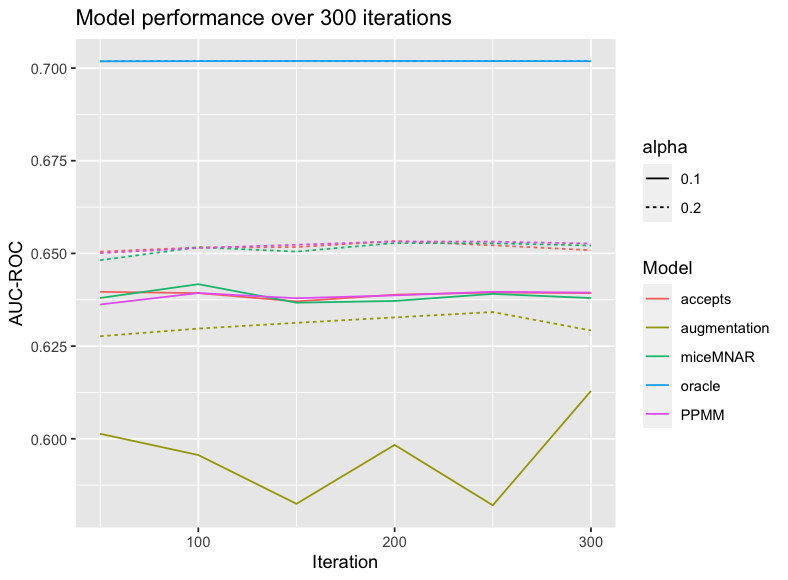
\includegraphics[width=0.5\linewidth]{Images/mix_8_2_alpha.png}
    \caption[Figure 1]{Parameters: $$\rowData{(1.5,0.8,0.8)}{(2,1,1)}{(0.1,0.2)}{0.3}{0.5}$$}
    \label{fig:acceptance_rate}
\end{figure}

The acceptance rate $\alpha$ proves to be one of the significant drivers of performance in the acceptance loop. A higher acceptance rate would essentially reduce the missing data thus reduces significantly the AUC values for all models. In both settings in \ref{fig:acceptance_rate} the novel methods \textit{PPMM} and \textit{miceMNAR} show minimal improvement over the model trained only on the accepts in the later iterations with performance being extremely similar over the initial iterations. 


% put one graph on changes of results of the PPMA model for a different phi
\subsubsection{Change in the $\phi$ value}

\begin{figure}[h!]
    \centering
    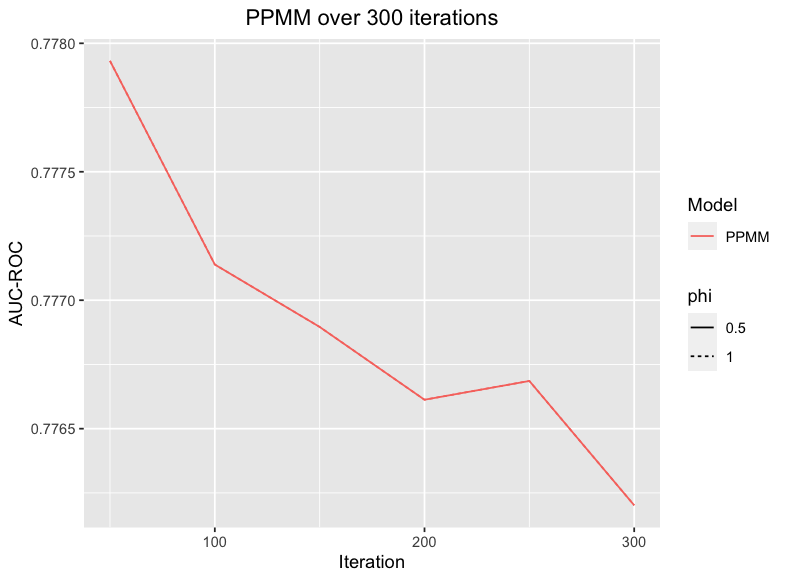
\includegraphics[width=0.5\linewidth]{Images/pmm_phi_2.png}
    \caption[Figure 2]{Parameters: $$\rowData{(1.2,0.6,0.6)}{(2,1,1)}{(0.2)}{0.3}{(0.5,1)}$$}
    \label{fig:phi_change}
\end{figure}

As already explained in \ref{ppma} $\phi$ represents the sensitivity parameter of the PPM model, essentially determining the missingness mechanism. A higher $/phi$ indicates a higher level of MNAR missingness. \ref{fig:phi_change} shows one of the simulations created with variation of the $\phi$ value and there is none effect visible. This could be due to the current implementation and the synthetic data used. The analysis of \cite{Andridge_Little_2020} shows that in the case of stronger proxies as defined in the pattern mixture model, $\phi$ has small to no effect.


\subsubsection{Change in mean values ($\mu$)}

Adjusting the mean values seems to have a large impact on the model performance. When the difference is very large, especially with 3 variables - which is implemented, so that Galimard works properly. With a diff from (0,0,0) + two noisy features drawn from the same distribution results in almost identical results in all cases. Slight differences are to be observed only compared to the oracle model (Oracle - 98.8 and all other models converge to 98.5 AUC ROC after 300 iterations of the loop)



\begin{figure}[h!]
    \centering
    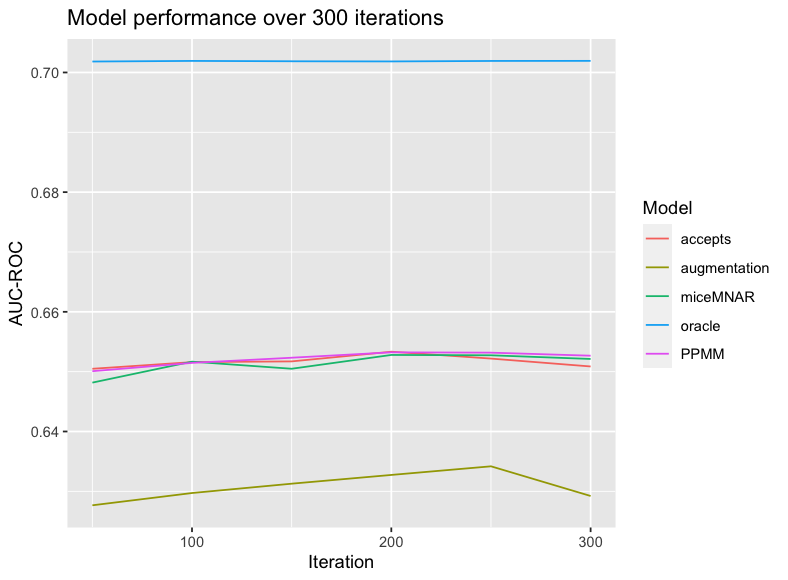
\includegraphics[width=0.5\linewidth]{Images/combination_8_3.png}\hfill
    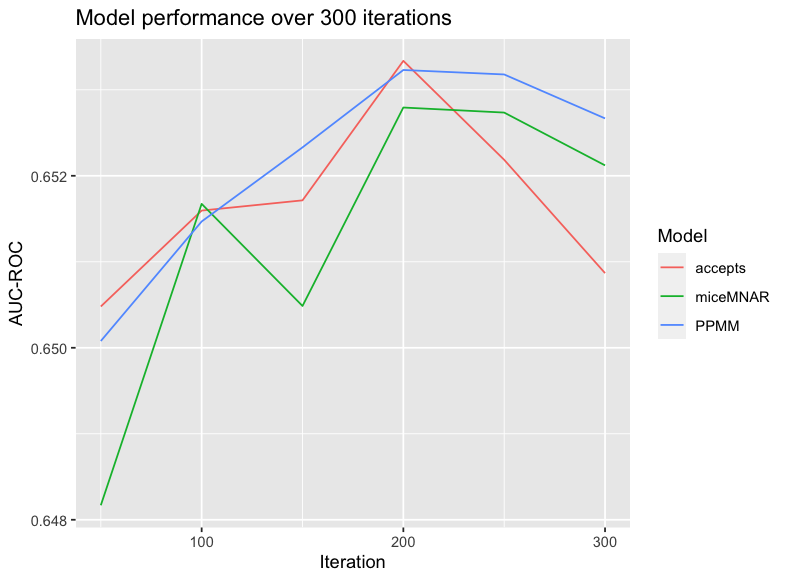
\includegraphics[width=0.5\linewidth]{Images/comb_8_side.png}
    \caption[Figure 3]{Parameters: $$\rowData{(1.5,0.8,0.8)}{(2,1,1)}{0.2}{0.3}{0.5}$$}
    \label{fig:combination_8}
\end{figure}

In the case of smaller differences in the mean values of the Gaussian distribution ($\mu^g$ and $\mu^b$), the results show a different behavior. In most of the parameter combinations with those characteristics \textit{MiceMNAR} and \textit{PPMM} delivered similar results to the model trained only on accepts, while augmentation showed a lower performance. Over 300 iterations the values fluctuate slightly with better AUC-ROC values for the novel techniques of less than 1 percent. \ref{fig:combination_8} shows the development over the 300 iterations (measurement done every 50 iterations) with the graph on the right-hand side showing only 3 of the models with close performance. 


\subsubsection{Change in covariance matrices}

A change in the covariance of the applicant's features is another interesting aspect. The more similar the covariances between the $bads$ and $goods$ the harder the classification task. This is also visible from \ref{fig:covariance_change} where there is a notable decrease in performance when using the same covariances when generating both $g$ and $b$ datasets in the case of the oracle model. Surprisingly the results for the novel methods seem to improve when the similarity of those cases. This is similar throughout different $\mu$ and $\alpha$ values. 

\begin{figure}[h!]
    \centering
    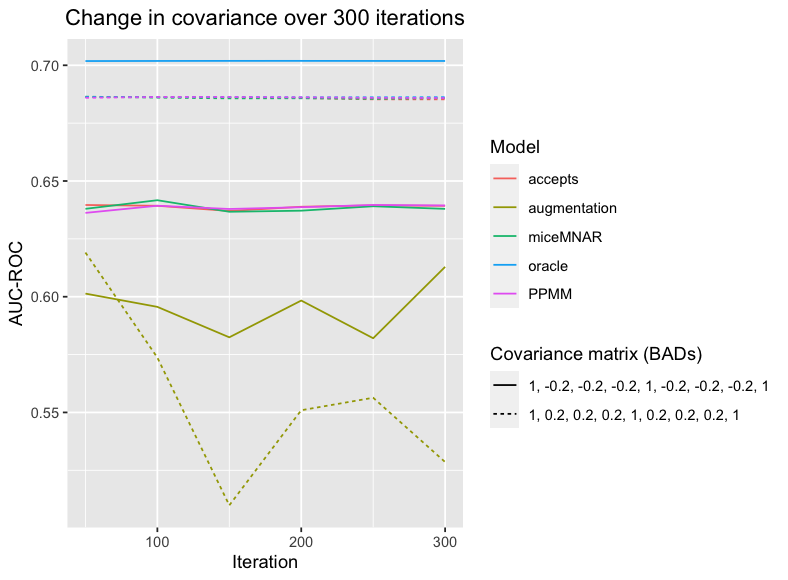
\includegraphics[width=0.5\linewidth]{Images/cov_2_5.png}
    \caption[Figure 4]{Parameters: $$\rowData{(1.5,0.8,0.8)}{(2,1,1)}{0.1}{0.3}{0.5}$$ $cov = (0.2,-0.2)$}
    \label{fig:covariance_change}
\end{figure}

The one model standing out is augmentation - augmentation delivers better results when covariances are similar for $\alpha$ = 0.2, but worsens its performance when covariances get more similar in the case of $\alpha$ = 0.1. 



\subsection{Acceptance loop with four variables}


The same acceptance loop was also implemented with two variables from the multivariate Gaussian distribution and two noisy features. This replicates the initial setup in the implementation of \cite{kozodoi_unpublished}. The results are more meaningful for this setup as because with a simple data generation the models often perform well in recognizing the pattern with few samples and the impact of missing data is limited. 
Parameters used were similar to the initial version of the loop described in \ref{parameters} except the number of variables given to the data generation function - in this case two instead of three in the initial version.
There were several interesting observations from this implementation of the acceptance loop. 

Interestingly, in \ref{fig:2_vars_aug} Augmentation shows itself as the most successful approach remaining close to the Oracle model even after 300 iterations, while the novel approaches and the model trained on the accepts show a declining performance with the increasing number of iterations. The parameters in this version of the acceptance loop opt in the case of medium mean proximity with $\mu^g = (1.2,0.6)$ and $\mu^b = (2,1)$ showing the mean values for $X_1$ and $X_2$ respectively. 


\begin{figure}[h!]
    \centering
    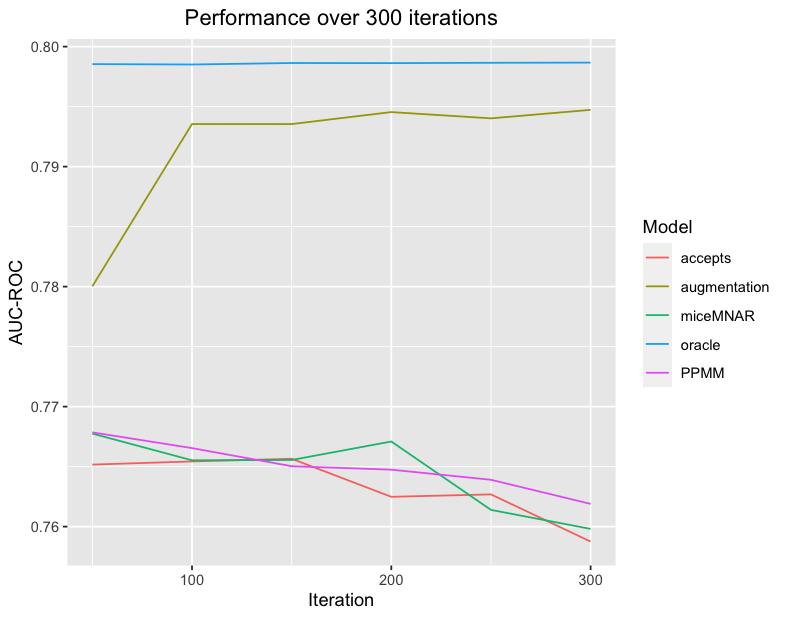
\includegraphics[width=0.5\linewidth]{Images/2_vars_comb_1.png}
    \caption[Figure 5]{Parameters: $$\rowData{(1.2,0.6)}{(2,1)}{0.1}{0.3}{0.5}$$
    $cov^b = -0.2$}
    \label{fig:2_vars_aug}
\end{figure}

In another run of the loop visible in \ref{fig:2_vars_drop_aug} \textit{MiceMNAR} and \textit{PPMM} managed to improve the performance over the \textit{accepted} based model while the model corrected by augmentation shows unstable behavior dropping surprisingly in performance in the final measurement (300. iteration).


\begin{figure}[h!]
    \centering
    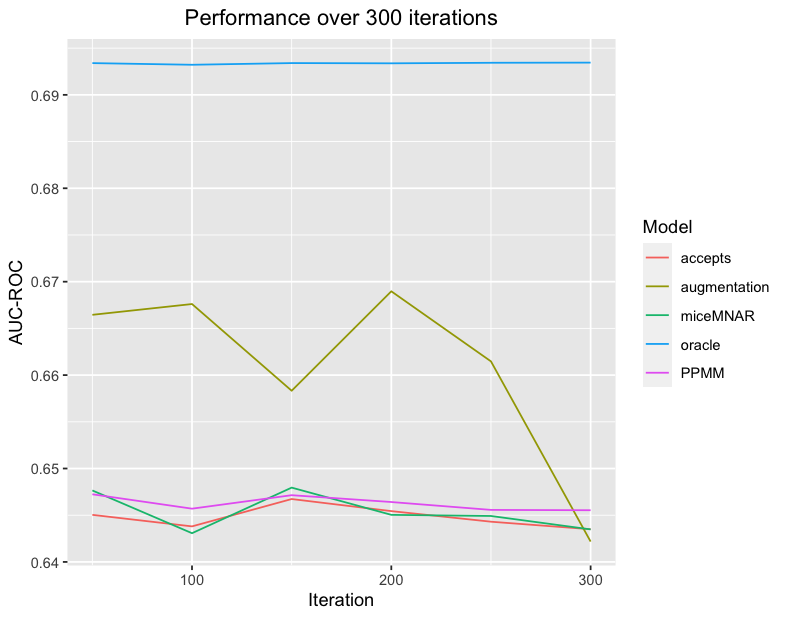
\includegraphics[width=0.5\linewidth]{Images/2_vars_cat_2.png}
    \caption[Figure 6]{Parameters: $$\rowData{(1.5,0.8)}{(2,1)}{0.1}{0.3}{0.5}$$ $cov^b = -0.2$}
    \label{fig:2_vars_drop_aug}
\end{figure}

PPMM and Galimard also performed well on some of the runs with a notable example in \ref{fig:2_vars_gal_pppmm}. \textit{PPMM} was stable and consistently outperforming the \textit{accepts-trained model}. \textit{MiceMNAR} showed a very unstable performance with serious peaks that are at times outperforming all the other models and coming close to the \textit{Oracle} model. In this particular run the covariance parameter was adjusted to the same values for both \textit{g} and \textit{b} populations.

\begin{figure}[h!]
    \centering
    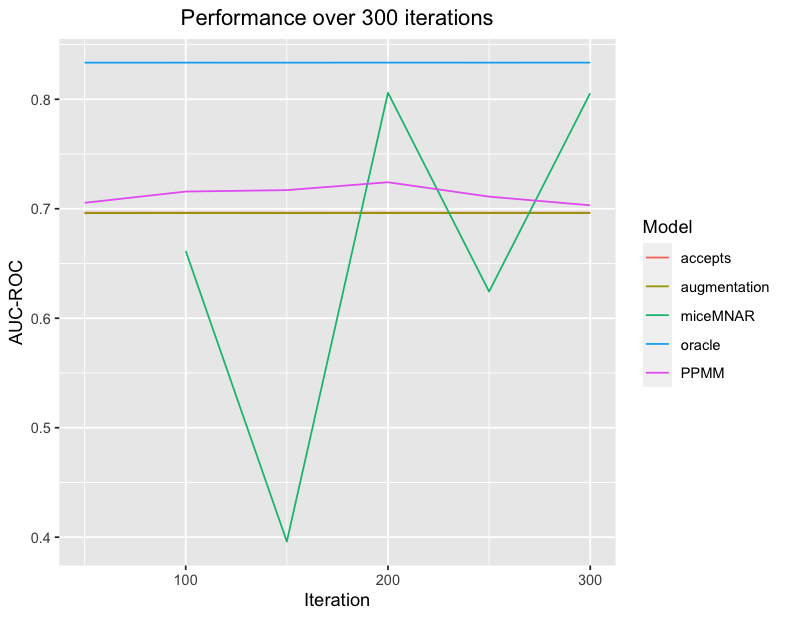
\includegraphics[width=0.5\linewidth]{Images/2_vars_comb_6.png}
    \caption[Figure 7]{Parameters: $$\rowData{(1,0.5)}{(2,1)}{0.1}{0.3}{0.5}$$ $cov^b = 0.2$}
    \label{fig:2_vars_gal_pppmm}
\end{figure}


\section{Conclusion}


In this thesis, we conducted an analysis of available novel missing data techniques and aimed at employing them in the context of Reject Inference. Through the usage of synthetic data in a simulation study and a sensitivity analysis, two novel approaches for dealing with MNAR missing data were tested. 

The findings uncover the benefits of using more complex missing data techniques in the field of Reject Inference. Some of the used techniques showed promising results in certain very limited settings and their potential application should be a matter of larger research. Even when the results are positive, they often seem unstable and random in the given simulation setting. Often theoretically and practically much simpler techniques that need fewer assumptions reach similar results. 
Limitations of the study include the limited availability of suitable data and for this reason the use of synthetic data. This may seriously limit the validity of the results. An additional limitation are series of assumptions for the use of those models including a rather theoretical justification for their usage. 

Another important note is the fact that those models are to be employed in a regulated environment where stability of results, but also explainability to a rather high degree are required.  
Future research could look into more of the MNAR techniques and estimate which of them are more realistically usable in the field of Reject Inference. 








\bibliographystyle{plain}
\bibliography{references}


    \newpage
\thispagestyle{empty}

\LARGE
Declaration of Academic Honesty
\vspace{1 cm}

\normalsize
I, Radoslav Evtimov, hereby declare that I have not previously submitted
the present work for other examinations. I wrote this work independently. All sources, including sources from the Internet, that I have reproduced in either an unaltered or modified form (particularly sources for texts, graphs, tables and images), have been acknowledged by me as such. I understand that violations of these principles will result in proceedings regarding deception or attempted deception.

\vspace{4 cm}

    

\raggedright\ Radoslav Evtimov\par \newline
Berlin, 07.03.2024




\end{document}